\documentclass[a4paper,10pt]{article}
\usepackage[utf8]{inputenc}
\usepackage{graphicx}
\usepackage{circuitikz}

%opening
\title{Curva caratteristica del diodo}
\author{Belliardo Federico, Marco Costa}

\begin{document}

\maketitle

\begin{abstract}
In questa esperienza si sono raccolte delle misure di tensione e di corrente relative ad un diodo in diverse condizioni di lavoro, utilizzando due diverse metodologie di misura, 
una automatizzata con Arduino e una manuale effettuata con due tester da laboratorio. I dati ottenuti sono stati \emph{fittati} utilizzando diverse procedure per ricavare i parametri caratteristici
di funzionamenti del particolare diodo utilizzato. In particolare si è misurata la resistenza asintotica del diodo per gradi tensioni e si è cercato di individuarne l'origine.
\end{abstract}

\section{Introduzione al diodo}
Il diodo è il primo componente non lineare che si incontra nel corso di laboratorio di fisica, il suo funzionamento si basa sui fenomeni elettrodinamici che occorrono quando due 
parti di silicio drogate rispettivamente con boro (p) e con fosforo (n). I risultato è che il diodo agisce come un raddrizzatore cioè lascia passare la corrente in un verso mentre la blocca
se collegato nel senso opposto, dunque i diodi sono dotati di polarizzazione, si diranno in polarizzazione diretta quando la corrente può scorrere e in polarizzazione inversa quando questa è bloccata. 
Delle considerazioni di meccanica statistica permettono di trovare una legge corrente tensione per il diodo, più dettagliata di quelle sopra esposta chiamata \emph{equazione di Shockley} che viene
in genere scritta come segue: 
\begin{equation}
 I = I_0 (e^{\frac{V}{\eta V_t}}-1)
\end{equation}
Dove $I_0$ viene chiamata corrente di saturazione inversa, $V_t$ è la tensione di threshold e $\eta$ è un fattore di forma.
Come si può dedurre dall'equazione, prendendo il limite $V \longrightarrow -\infty$ la corrente di saturazione inversa in modulo è quella che attraverserebbe il diodo 
collegandolo con polarità scambiata ad una differenza di potenziale infinita.
La tensione $V_t$ è uguale nel modello di Shockley a $\frac{k_B T}{e}$, alla temperatura ambiente di $300 K$ vale $k_B T = \frac{1}{40} eV$ dunque $V_t = 26 mV$ circa come valore numerico.
Il fattore di forma è invece in genere compreso tra 1 e 2.
Il parametro $\eta$s è chiamato fattore di forma 
I diodi presentano una linea argentata in corrispondenza del catodo (come in figura), in seguito è anche riportato il simbolo circuitale del diodo, che è una freccia indicante 
la direzione di scorrimento della corrente.

\begin{figure}[!htb]
\begin{center}
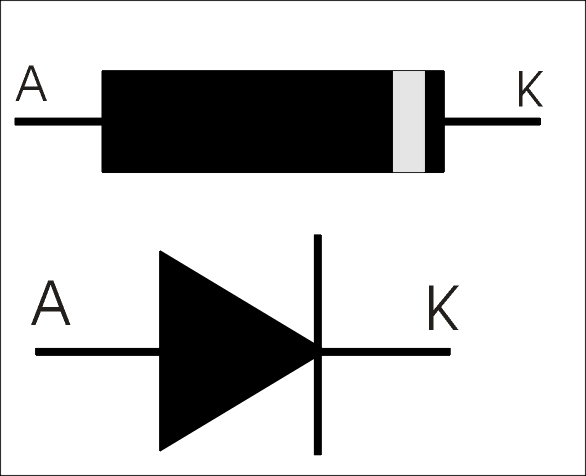
\includegraphics[width=0.3\textwidth]{diodo.jpg}
\end{center}
\label{figura_di_esempio}
\end{figure}

\section{Misure con Arduino}
Per misurare le grandezze che compaiono nella legge di Shockley si è utilizzato un sistema automatizzato di raccolta dati gestito da Arduino. 
Una delle porte di Arduono era configurata in modalità PWM

\begin{circuitikz}
 \draw  (0,0) to[R, l = $R$] (2,0);
 \draw  (2,0) to[R, l = $R_D$] (4,0);
 \draw	(2,0) to[short, -o] (2,2);
 \draw	(4,0) to[short, -o] (4,2);
 \draw	(2,0) to[C, l = $C$] (2,-2);
 \draw	(2,-2) to[short] (4, -2);
 \draw	(4, 0) to[diode] (4,-2);
\end{circuitikz}


\section{Analisi dei dati}

\section{Grafici e fit}
I dati raccolti con Arduino e linearizzati non evidenziano alcuna significativa deviazione dalla legge di Shockley, infatti per trovare una tale deviazione si sono dovute eseguire misure a voltaggi
molto più elevati.

\section{Misure ad alte tensioni}

\section{Misure}

\end{document}
